\documentclass[11pt]{article}
\pdfobjcompresslevel=0 % force classic uncompressed xref table (avoids MiKTeX broken-xref-stream bug)
\usepackage[margin=2.3cm]{geometry}
\usepackage[T1]{fontenc}\usepackage{lmodern}
\usepackage{amsmath,amssymb,mathtools}
\usepackage{tcolorbox}\tcbuselibrary{skins,breakable}
\usepackage{booktabs}\usepackage{array}\usepackage{enumitem}
\usepackage{fancyhdr}\setlength{\headheight}{14.5pt}
\usepackage{parskip}\usepackage{xcolor}\usepackage{hyperref}
\usepackage{tikz}\usetikzlibrary{arrows.meta,positioning}

% ---- DTF chain-flow identity (shared across the trilogy) --------------------
\definecolor{dtfblue}{HTML}{1a1a2e}\definecolor{dtflight}{HTML}{0f3460}
\definecolor{boxblue}{HTML}{e8f4f8}\definecolor{knownblue}{HTML}{1a3a6e}
\definecolor{chainbg}{HTML}{f7f9fc}\definecolor{chainframe}{HTML}{c0cce0}
\definecolor{cbKnownBg}{HTML}{E9E9FA}\definecolor{cbKnownFr}{HTML}{8E97C9}
\definecolor{cbNodeBg}{HTML}{F4F5F8}\definecolor{cbNodeFr}{HTML}{CDD2DB}
\definecolor{cbAssumeBg}{HTML}{FBEBEB}\definecolor{cbAssumeFr}{HTML}{C0392B}
\definecolor{cbResultBg}{HTML}{FBF4D2}\definecolor{cbResultFr}{HTML}{C8A21E}
\definecolor{cbTagBg}{HTML}{E2F1EF}\definecolor{cbTagFr}{HTML}{4FA295}
\definecolor{cbArrow}{HTML}{8A93A6}\definecolor{cbPyBg}{HTML}{ECEFF4}

\tcbset{
  keybox/.style={enhanced,breakable,colback=boxblue,colframe=dtfblue,boxrule=0.8pt,
    arc=3pt,left=10pt,right=10pt,top=8pt,bottom=8pt},
  cbflow/.style={enhanced,arc=3.5pt,boxrule=0.7pt,left=12pt,right=12pt,top=10pt,bottom=10pt,
    before skip=4pt,after skip=4pt},
}
\newcommand{\chainarrow}{\vspace{1pt}\centerline{\tikz{\draw[-{Latex[length=2.6mm,width=2.2mm]},
  line width=1pt,cbArrow](0,0.28)--(0,0);}}\vspace{1pt}}
\newcommand{\known}[2]{\begin{tcolorbox}[cbflow,colback=cbKnownBg,colframe=cbKnownFr]
  \centering\(\displaystyle #1\)\\[3pt]{\color{knownblue}\small[\,\textit{known: #2}\,]}\par
  \nobreak\vspace{1pt}\hfill{\tiny\color{gray}Known}\end{tcolorbox}}
\newcommand{\knowntext}[2]{\begin{tcolorbox}[cbflow,colback=cbKnownBg,colframe=cbKnownFr]
  \small #1\par{\color{knownblue}\small[\,\textit{known: #2}\,]}\par
  \nobreak\vspace{1pt}\hfill{\tiny\color{gray}Known}\end{tcolorbox}}
\newcommand{\assume}[1]{\chainarrow\begin{tcolorbox}[cbflow,colback=cbAssumeBg,colframe=cbAssumeFr]
  {\color{cbAssumeFr}\bfseries[DTF input:]\ }{\color{cbAssumeFr}\small #1}\par
  \nobreak\vspace{1pt}\hfill{\tiny\color{gray}DTF input}\end{tcolorbox}}
\newcommand{\nodetext}[1]{\chainarrow\begin{tcolorbox}[cbflow,colback=cbNodeBg,colframe=cbNodeFr]
  \small #1\par\nobreak\vspace{1pt}\hfill{\tiny\color{gray}Derivation}\end{tcolorbox}}
\newcommand{\dtfresult}[2]{\chainarrow
  \begin{tcolorbox}[cbflow,colback=cbResultBg,colframe=cbResultFr,boxrule=1.3pt]
  \centering\(\displaystyle #1\)\par\nobreak\vspace{1pt}\hfill{\tiny\color{gray}DTF result}\end{tcolorbox}\chainarrow
  \begin{tcolorbox}[cbflow,colback=cbTagBg,colframe=cbTagFr]
  \centering{\itshape\color{dtflight}#2}\par\nobreak\vspace{1pt}\hfill{\tiny\color{gray}Takeaway}\end{tcolorbox}}
\newcommand{\pychip}[2]{{\footnotesize\colorbox{cbPyBg}{\ttfamily\,#1\,}\,{\color{gray}$\to$ #2}}}
\newcommand{\resultpy}[3]{\chainarrow
  \begin{tcolorbox}[cbflow,colback=cbResultBg,colframe=cbResultFr,boxrule=1.3pt]
  \centering\(\displaystyle #1\)\par\smallskip\centering\pychip{#2}{#3}\par
  \nobreak\vspace{1pt}\hfill{\tiny\color{gray}DTF result --- verified}\end{tcolorbox}}
\newcommand{\oneobject}[2]{\begin{tcolorbox}[enhanced,colback=white,colframe=black,boxrule=1.3pt,arc=3pt,
  left=10pt,right=10pt,top=7pt,bottom=7pt,before skip=4pt,after skip=4pt]
  {\bfseries One object, seen here as: #1}\\[2pt]{\small #2}\end{tcolorbox}}
\newenvironment{chainbox}{\par\addvspace{4pt}\noindent\ignorespaces}{\par\addvspace{4pt}}
\newcommand{\chainhead}[2]{\subsection*{Chain #1\quad\normalfont\itshape #2}}
\newcommand{\setup}[1]{\noindent\emph{#1}\par\smallskip}

\hypersetup{colorlinks=true,linkcolor=knownblue,citecolor=knownblue,urlcolor=knownblue,
  pdftitle={The Distorted Time Framework, Volume I: The Forgotten Primitive},
  pdfauthor={William de Dufour}}
\pagestyle{fancy}\fancyhf{}
\fancyhead[L]{\small\itshape Distorted Time Framework --- Volume I}
\fancyhead[R]{\small\itshape The Forgotten Primitive}
\fancyfoot[C]{\small\thepage}\renewcommand{\headrulewidth}{0.4pt}

\begin{document}

\begin{center}
{\large\bfseries The Distorted Time Framework\\[3pt]
\normalsize Volume I --- \itshape The Forgotten Primitive}\\[6pt]
{\small A Time-First Assembly of Physics}\\[10pt]
{\normalsize William de Dufour}\\[2pt]
{\small\itshape Independent Researcher, Austin, TX}\\[2pt]
{\small\texttt{billd.dtf@gmail.com}}\\[2pt]
{\small ORCID: \href{https://orcid.org/0009-0008-3470-1231}{0009-0008-3470-1231}}\\[2pt]
{\small\url{https://github.com/billd-dtf/Distorted-Time-Framework}}\\[3pt]
{\small Version 8}\\[3pt]
{\small\href{https://doi.org/10.5281/zenodo.21659853}{\texttt{DOI: 10.5281/zenodo.21659853}}}
\end{center}

\begin{abstract}
This is an \emph{organizing-principle} account of physics, in the sense Laughlin and Pines gave the
term~\cite{LaughlinPines2000}: its subject is not a new force, particle, or equation, but the ontological
status of one quantity already in the equations---the local \emph{rate} of time, the ADM lapse of general
relativity, reclassified as physical rather than discarded as a gauge coordinate. Taken as the single
primitive, it \emph{organises} the rest: quantum indefiniteness, spacetime geometry, temporal orientation,
and measurement stop being separate frameworks and become faces of one thing. The organising fact is
that \emph{space is what time radiates}: because radiation lives in the spatial sector, the clock rate
itself carries zero propagating degrees of freedom, so promoting time to a field adds no breathing mode,
introduces no ghost, and breaks no Lorentz invariance---by structure, not by tuning. From this the volume
reads out, in short explicit chains, a native temporal orientation, the equivalence principle as a single identity, and
exactly two tensor gravitational-wave polarisations; and it locates one clock-definiteness surface beneath
two standing problems at once---quantum measurement and the black-hole core, the same transition run in
opposite directions. Volumes~II and~III carry this into gravity and the singularity, and into the Born rule
and measurement. Every tested prediction of quantum mechanics and general relativity is left intact, and no
particle, force, or new fundamental constant is added: the claim is a \emph{reorganisation}, not a replacement---and,
deliberately, not a unification of the forces.
\end{abstract}

\smallskip
\noindent{\small\textbf{Keywords:} time as primitive; ADM lapse; ontology of physics; preferred foliation;
problem of time; organizing principles; foundations of quantum gravity.}

\bigskip

\noindent For a century we have been \emph{decompiling} nature --- reverse-engineering the running
universe back to its source code, and doing it superbly: quantum mechanics, general relativity,
quantum field theory, each accurate past any reasonable doubt. But in the decompile we treated
\emph{time} as scaffolding rather than source: an external parameter in QM, a gauge coordinate in
GR, discarded either way. This volume asks what happens when time's local \emph{rate} is put back as
the one physical primitive --- and lets the structure of physics reassemble around it. This is the gap
Laughlin and Pines named --- reductionism superb at the fundamental laws, far weaker at the
\emph{organizing principles} that say how their consequences cohere, which they placed at the centre of
what physics has left to do~\cite{LaughlinPines2000}. This volume offers time's rate as one such principle:
a \emph{reclassification} of a quantity already in the equations (the ADM lapse~\cite{ADM1962}), not a new
field bolted onto general relativity. What that organises, and what it pointedly does \emph{not} claim, the
box below states plainly.

\noindent A physicist hears ``time as a field'' and reaches, rightly, for the three failures that have
buried every previous attempt: a new \emph{propagating mode} (a scalar or breathing gravitational wave
no detector sees), a broken \emph{Lorentz invariance} (a preferred frame the experiments have closed
off), and a \emph{ghost} (the conformal mode's wrong-sign kinetic energy). One fact meets all three, and
it is this volume's lead: \textbf{space is what time radiates}. An extent is a period thrown off at $c$
($\lambda_C=c\,T_C$) --- so the \emph{radiative} sector \emph{is} space, and the rate of time itself does
not propagate at all ($\pi_u\equiv0$, exact: the action carries no $\dot u$). The classical no-go theorems
assume a scalar that \emph{propagates} in the continuum; here $u$ is a \emph{constraint}, and they lose
their grip. The three legs are not equally strong, though, and grading them is more convincing than
flattening them:
\begin{itemize}[leftmargin=1.5em,itemsep=2pt,topsep=3pt]
  \item \textbf{No new propagating mode --- structural, and checked.} $u$ carries zero degrees of freedom
    (Appendix~A). The \emph{frame} field does propagate, carrying the two tensor polarisations; what is new
    here adds none.
  \item \textbf{No ghost --- structural.} A field entering the action with no $\dot u$ has no kinetic term,
    so it cannot carry the wrong sign of one. The objection cannot be posed, rather than being evaded.
  \item \textbf{Lorentz invariance --- structural, and now checked.} $\alpha_1,\alpha_2$ are nonzero only
    when a theory has something draggable relative to matter --- an independently dynamical preferred-frame
    field, whose kinetic couplings \ae ther theories must tune. Every such coupling needs a $\dot u$; DTF has
    none, so it is not at a tuned point but outside that parameter space entirely. And the structural claim
    now carries the explicit calculation that could have contradicted it: boosting the metric at the first
    post-Newtonian order where a preferred-frame term can appear returns exactly the Lorentz-invariant
    coefficient, with the would-be $\alpha_1$ term absent (\S A.3).
\end{itemize}
\noindent All three now rest on the same absence of a $\dot u$ term. What remains genuinely contingent is
narrower and is named where it bites: the conformally-flat scheme by which the metric is \emph{reconstructed}
for computation beyond 1PN (Volume~II), which limits calculation, not these three claims.

\textbf{What kind of claim this is --- an organizing principle, not a new force.}\enspace Laughlin and
Pines~\cite{LaughlinPines2000} drew a line physics rarely states aloud: reductionism has been superb at the
\emph{fundamental laws} and far weaker at the \emph{organizing principles} --- the higher-level facts that
say how the laws' consequences hang together --- and they argued the second, not the first, is the work that
remains. DTF is offered squarely as one such principle, and its ambition is set by that: it adds no
particle, no force, and no free parameter, and it leaves every tested prediction of quantum mechanics and
general relativity exactly where it found them. It is therefore \emph{not} a grand unification, and
\emph{not} a ``theory of everything'' in the usual sense of one dynamics for all the forces --- and it does
not pretend to be.
\smallskip
\noindent What it unifies is one level up: the disjoint \emph{frameworks}. Quantum theory keeps time an
external parameter; general relativity keeps it a gauge label; thermodynamics grants it a direction;
measurement theory bolts on a collapse. Each framework's central unsolved problem is what is left dangling
by never saying what the \emph{rate} of time \emph{is}. Restore it as the one primitive and those problems
--- the problem of time, the definiteness of measurement, the postulated Born rule, the singularity ---
stop being four mysteries and become one omission seen in four sectors, resolved by the \emph{same}
machinery rather than four separate patches. That mutual consistency, not any single chain, is the claim;
each chain below is only where it is checked in one sector. Its sharpest single expression is Chain~8: the
surface where the clock loses definiteness is \emph{one} surface, and quantum measurement (a clock
\emph{becoming} definite) and the black-hole core (a clock \emph{de-emerging}) are that one surface crossed
in opposite directions. And the sectors are stitched at one place --- the \emph{proper now}, the preferred
slice a non-propagating clock rate forces ($\pi_u\equiv0$): where gravity solves its field, where entangled
systems share a present, and where a relativistic quantum diffusion would run. It is the real, empirically
silent present that physics has reached for sector by sector --- cosmic time, the collapse slice, the
Bohmian foliation --- and that here simply \emph{falls out}. That restored now is the second half of the
claim.

\begin{tcolorbox}[keybox,unbreakable]
\textbf{The three commitments --- and the core that follows.}\enspace The framework is built forward from
three, stated plainly:
\begin{enumerate}[leftmargin=1.6em,itemsep=1pt,topsep=3pt]
  \item \textbf{Time is primitive} --- its local \emph{rate} $u$ is the one physical thing.
  \item \textbf{Space is time's radiation} --- an extent is a period thrown off at $c$ ($\lambda_C=c\,T_C$);
    the \emph{radiation rule} compiles a rate field into distances (Chain~5, and the example below).
  \item \textbf{There is a proper now} --- one real, shared present.
\end{enumerate}
\noindent The first is \emph{asserted}; the second is \emph{shown} (Chain~5), and with it the three rows
(Row~0 timeless substrate $\to$ Row~1 the clock $\to$ Row~2 space). The third is \emph{declared} --- DTF's
\emph{second} posit, and the best-motivated one in physics: DTF takes one slice, the
constant-mean-curvature (constant-$u$) section, to be ontologically real. It is \emph{not} forced by energy
conservation --- the Hamiltonian constraint $\hat H\Psi=0$ holds on \emph{every} slice --- but it is the
slice on which that constraint is uniquely well-posed (Lichnerowicz--York~\cite{Lichnerowicz1944,York1972}), the one numerical relativity
converges on, the foliation Bohmian mechanics needs, and the output of shape dynamics. One posit, four
sectors. So the framework carries \emph{two} posits --- a definite clock rate, and a real constant-$u$
slice --- an unusually lean ontology; and the same conserved Row-0 energy is the clock ($E=\hbar\omega_C$)
and Row~1's temporal orientation ($\tau$ monotone).
\pychip{DTF\_row0\_energy\_to\_now.py}{conserved energy $\to$ unique $u$ on the slice; a rate well $\to$ induced length $+$ osmotic drift}
\end{tcolorbox}

\noindent Volume~I constructs the ontology from the ground up; Volumes~II (gravity, the singularity)
and~III (the Born rule, and the reading of the quantum) carry it into each sector. The method is uniform
and shown in every step: state a minimal condition on the primitive, and read off the object it forces.

\begin{center}
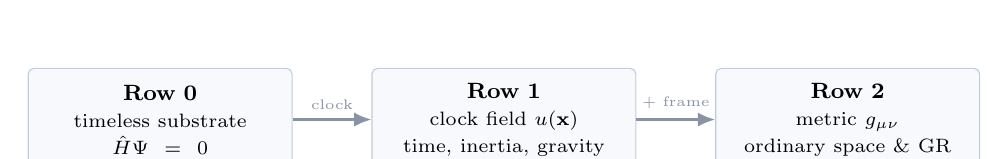
\begin{tikzpicture}[font=\footnotesize,node distance=10mm,
  rowbox/.style={draw=chainframe,fill=chainbg,rounded corners=2pt,align=center,inner sep=5pt,
    minimum height=13mm,text width=30mm},
  rowar/.style={-{Latex[length=2.2mm,width=1.8mm]},cbArrow,thick}]
\node[rowbox](r0){\textbf{Row 0}\\[2pt]\scriptsize timeless substrate\\\scriptsize $\hat H\Psi=0$};
\node[rowbox,right=of r0](r1){\textbf{Row 1}\\[2pt]\scriptsize clock field $u(\mathbf x)$\\\scriptsize time, inertia, gravity};
\node[rowbox,right=of r1](r2){\textbf{Row 2}\\[2pt]\scriptsize metric $g_{\mu\nu}$\\\scriptsize ordinary space \& GR};
\draw[rowar](r0)--(r1)node[midway,above,font=\tiny]{clock};
\draw[rowar](r1)--(r2)node[midway,above,font=\tiny]{$+$ frame};
\end{tikzpicture}
\end{center}

\noindent\textbf{How to read the chains.}\quad Each result is built as a short vertical derivation:
\begin{center}
{\footnotesize\colorbox{cbKnownBg}{known}} $\to$ {\footnotesize\colorbox{cbAssumeBg}{DTF input}} $\to$
{\footnotesize\colorbox{cbNodeBg}{derivation}} $\to$ {\footnotesize\colorbox{cbResultBg}{result\,(+\,\texttt{.py})}} $\to$
{\footnotesize\colorbox{cbTagBg}{takeaway}}
\end{center}
\noindent One line sets each chain up; the math does the rest.

\bigskip

\textbf{The ledger: what the ontology removes.}\enspace The case for a reorganisation is not that it
predicts a new number --- it leaves every successful one untouched --- but that the left column below,
a collection of separate postulates, coincidences, and standing problems, is replaced by the right,
which is shorter. Each row is argued in the chain or volume named; this is the economy at a glance.
\smallskip
\begin{center}\small\renewcommand{\arraystretch}{1.25}
\begin{tabular}{@{}>{\raggedright\arraybackslash}p{5.0cm}>{\raggedright\arraybackslash}p{8.4cm}c@{}}
\toprule
\textbf{Standard package} & \textbf{DTF reading} & \textbf{where}\\
\midrule
Preferred foliation --- an \emph{extra postulate} (relativistic Bohm) & the slice gravity already solves
its field on ($\pi_u\equiv0$); not added for the quantum & Ch.\,7,\,Vol III\\
Equivalence principle --- a \emph{coincidence} awaiting a test & one identity: inertia and the well it
digs are the same rate $\omega_C$ & Ch.\,6\\
Born rule --- a \emph{measurement axiom} & the equilibrium of the conserved location-density & Vol III\\
Wavefunction collapse --- a \emph{fundamental process} & unnecessary: the particle is already definite
(only \emph{which} outcome stays owed) & Vol III\\
Singularity --- \emph{infinite curvature}, theory's end & the boundary where temporal language
de-emerges, at finite density & Vol II\\
Problem of time --- \emph{recover} time from a timeless equation & time's rate is the primitive; the
timeless equation is Row 0, its floor & Ch.\,1--2\\
\bottomrule
\end{tabular}
\end{center}
\smallskip
\noindent The ledger removes postulates; it does not claim to have paid every debt. Two remain, named
where they bite: \emph{which} single outcome a measurement selects (Vol III), and the microscopic origin
of clock definiteness (Chain 8). Both are standing debts of the standard package too --- carried here,
not hidden.

\bigskip

\clearpage
\chainhead{1}{The floor has no clock}
\setup{Strip the world back to its ground: what remains when no clock is running?}
\begin{chainbox}
\knowntext{Canonical quantum gravity has a timeless ground: the Wheeler--DeWitt constraint
$\hat H\Psi=0$ holds with no external parameter $t$ to evolve against.}{DeWitt 1967~\cite{DeWitt1967}}
\dtfresult{\hat H\Psi=0\ \Longrightarrow\ \textbf{Row 0 (timeless)}}
{No ``when.'' Relations hold all at once; nothing is earlier or later --- and with no time to change
against, $\hat H\Psi=0$ is not an evolution law but the \emph{energy constraint}: energy is Row~0's one
conserved invariant. This is the floor everything else is built on, and (Chain~7) the fixed content that
fixes the now.}
\end{chainbox}

\chainhead{2}{A definite clock makes time --- and points it}
\setup{Condition one definite clock-rate on the floor. Its reading is the first ``later.''}
\begin{chainbox}
\assume{a local clock-rate field $u(\mathbf x)>0$ becomes definite on Row~0. (This is the one posit;
its microscopic origin is left open, and named in the ledger.)}
\nodetext{the reading accumulates,
\[ \tau=\int u\,dt, \]
and because $u>0$ it is strictly monotone --- it can only grow.}
\dtfresult{\tau=\textstyle\int u\,dt\ \text{monotone}\ \Longrightarrow\ \textbf{Row 1}+\text{a native temporal orientation}}
{Time is the clock's reading, not a backdrop it runs against. Its one-way growth gives Row~1 a native
\emph{orientation} --- an ordering, for free. That is \emph{not} yet the thermodynamic arrow, which needs a
statement about initial conditions (the past hypothesis) this framework does not supply.}
\end{chainbox}

\chainhead{3}{The reading is a phase; its straightest path is Fermat's}
\setup{Read the clock reading as a quantum phase, and ask which path it makes stationary.}
\begin{chainbox}
\known{\Phi=-\omega_C\,\tau,\qquad \tau=\int d\tau\ (\text{proper time};\ \textstyle\int u\,dt\ \text{at rest}),\qquad \omega_C=\frac{mc^2}{\hbar}}
{internal phase of any quantum, re-read as a clock reading}
\nodetext{the rule is to extremise the accumulated \emph{proper time},
\[ \delta\!\int d\tau=0,\qquad d\tau=\sqrt{u^2dt^2-dx^2/c^2}, \]
whose geodesics are free fall. For a slow body,
\[ \int d\tau\ \approx\ \int\!\Big(u-\frac{v^2}{2c^2u}\Big)dt; \]
dropping the kinetic term leaves $\delta\!\int u\,dt=0$, the \emph{static} (Fermat) reduction that Chain~6's
force $=-c^2\nabla u$ lives in.}
\dtfresult{\text{one object}\ \ \Phi=-\omega_C\!\int d\tau,\qquad \text{one method}\ \ \delta\!\int d\tau=0}
{Everything below is this single object, moved by this single rule: extremise accumulated \emph{proper
time}. Its rest-frame reduction $\delta\!\int u\,dt=0$ is the static limit.}
\end{chainbox}

\clearpage
\chainhead{4}{One object, four faces}
\setup{Read that one stationary phase four ways. Each is a textbook law; all are the same expression.}
\begin{chainbox}
\known{S=\hbar\Phi=-mc^2\!\int d\tau}{the action is the phase (accumulated proper time)}
\nodetext{differentiate $S$ (inertia), extremise $S$ (gravity), ride $\nabla S$ (guidance), sum
$e^{iS/\hbar}$ over histories (path integral) --- four questions asked of one $S$.}
\resultpy{\underbrace{\mathbf p=\nabla S}_{\text{inertia}}\;=\;\underbrace{\delta\!\int d\tau=0}_{\text{geodesic}}
\;=\;\underbrace{\mathbf v=\nabla S/m}_{\text{pilot wave}}\;=\;\underbrace{\textstyle\sum e^{iS/\hbar}}_{\text{path integral}}}
{DTF\_phase\_unification.py}{one $S$, four laws}
\end{chainbox}
\oneobject{inertia \& the pilot wave}{Both read the one phase $\Phi=-\omega_C\tau$, and \emph{neither
carries $G$}. Inertia \emph{is} the rate $\omega_C$ --- the mass $m=\hbar\omega_C/c^2$, linear in $m$,
definitional: the clock's ticking, not a mechanism to derive. Guidance is the \emph{space}-face gradient
$\nabla S$ --- $\hbar$-coupled, and it \emph{survives even at $u\equiv1$} (a perfectly flat clock field).
The two are tied because the momentum \emph{is} that gradient, $\mathbf p=\nabla S=m\mathbf v$: one clock,
read as its rate and as the gradient it lays down. What is \emph{neither} of these --- the $G$-coupled
well the rate digs in $u$, $\sim(m/m_P)^2$ --- is gravity. The split runs on through Volumes~II and~III.}

\noindent\textbf{One caution, held to across the trilogy.}\enspace These four faces are all readings of the
one \emph{phase} $S$ --- the classical Hamilton--Jacobi/WKB level, at which the quantum potential is
suppressed. The \emph{amplitude} half that carries the quantum content --- continuity for $|\psi|^2$, the
quantum potential, and with it the Born rule --- is Volume~III's subject, and there it is \emph{reduced},
not derived. ``One object, four faces'' is a statement about the \emph{phase} sector; it is not a
derivation of quantum mechanics, and none is claimed here.

\clearpage
\chainhead{5}{Space is what time radiates}
\setup{The phase read along time gives a period; read along space it gives an extent. One bridge, $c$, ties them --- and that one bridge carries the rest of the volume.}
\begin{chainbox}
\known{E\,T_C=h\ \ (\text{time face}),\qquad E\,\lambda_C=hc\ \ (\text{space face})}
{Planck/Compton relations, one on each axis}
\nodetext{the two anchors differ only by $c$:
\[ \lambda_C=c\,T_C, \]
an extent is a period radiated at $c$. An orientation (frame) field compiles these extents into Row-2
geometry --- so the \emph{radiative} sector is space, while time's rate $u$ is the non-propagating source.}
\nodetext{the Compton relations make $\lambda_C/T_C=c$ \emph{identically}, the same for every mass ---
one exchange rate for all matter. This is a consistency restatement, not a derivation: Lorentz
invariance enters as the premise that the interval is
\[ d\tau^2=u^2dt^2-\frac{dx^2}{c^2} \]
with $c$ universal. What DTF adds is the \emph{reading} of that premise --- $c$ as the rate at which
space is made from time.}
\dtfresult{\lambda_C=c\,T_C\ \Longrightarrow\ \textbf{Row 2: space as time's radiation}}
{Space is not a second primitive; it is what time throws off at $c$. Two consequences carry the rest of
the volume: \emph{(i)} the ontology \emph{reads} Lorentz invariance as the signature of one universal
exchange rate (the interval is assumed, not derived); \emph{(ii)} radiation lives in \emph{space}, so
time's rate $u$ does not propagate --- there is no ``time wave.'' (Why exactly three dimensions:
Volume~II.)}
\resultpy{g_{00}=-u^2\ (\text{time}),\qquad \gamma_{ij}=(2-u^2)\,\delta_{ij}\ (\text{space}),\qquad -g_{00}+\gamma=2}
{DTF\_row0\_energy\_to\_now.py}{radiation rule: space is time's complement, $=$ GR to leading order}
\end{chainbox}
\noindent\textbf{The radiation rule, explicit.}\enspace This is the map ``space from the rate'' in one
line: what time's rate gives up, space takes. In a well ($u^2<1$) time slows and space stretches by exactly
the complement, $\gamma_{ij}=(2-u^2)\delta_{ij}$ --- reproducing general relativity's isotropic spatial
metric \emph{exactly to 1PN} (leading order in $u-1$; the full nonlinear map is Volume~II's IWM/CFC scheme).
Space is not compiled by a second law; it is the ledger balance of the one rate.
\oneobject{time \& space --- the proper-time interval}
{$\displaystyle d\tau^2=\underbrace{u^2dt^2}_{\text{time: the now}}-\underbrace{dx^2/c^2}_{\text{space: the radiation}}$.\;
The preferred now is the \emph{time}-face; Lorentz invariance is the \emph{space}-face; $c$ is the hinge.
A preferred slice and exact relativity are not in tension --- they are two readings of one interval.}

\chainhead{6}{Gravity is the shape of the clock field}
\setup{A slow body falls down the gradient of time's rate. Make that rate primitive, and gravity is its shape.}
\begin{chainbox}
\known{g_{00}=-u^2,\qquad \ddot{\mathbf x}=-c^2\nabla u\ \ (\text{slow body})}
{Newtonian limit of GR: gravity is the curvature of \emph{time}}
\assume{promote $u$ from consequence to primitive; the one reparametrization-invariant action
carries no $u$ time-derivative.}
\nodetext{then $u$ is non-propagating,
\[ \pi_u\equiv0, \]
and its field law is forced (not tuned).}
\dtfresult{\nabla^2 u=\tfrac{4\pi G}{c^2}\rho,\qquad \text{static force}=-c^2\nabla u}
{Gravity is the shape of the clock-rate field, sourced instantaneously through a constraint --- no
force carrier. And promoting \emph{time} to a field can neither add a wave nor break relativity --- not
as something to be checked, but \emph{by Chain~5}: radiation is space, time's rate $u$ does not
propagate, and $c$ is universal. The box below turns this into numbers. Full derivation: Volume~II.}
\end{chainbox}
\oneobject{inertia \& gravity}{One rate $\omega_C$: it \emph{is} the inertia (linear in $m$,
definitional), and it \emph{sources} the gravitational well in $u$ (the $G$-coupled $\sim(m/m_P)^2$
dent), whose extremum is free fall. The equivalence principle is that single identity --- not a
coincidence awaiting a test, and not two things whose equality needs explaining.}

\clearpage
\chainhead{7}{The shared present: the proper now}
\setup{DTF's second posit: one slice is real. It is a declaration --- and the best-motivated one in physics.}
\begin{chainbox}
\assume{\textbf{Posit 2:} the constant-$u$/CMC slice is ontologically real. Not \emph{forced} --- $\hat H\Psi=0$ holds on every foliation --- but it is the slice on which the energy constraint is uniquely well-posed (Lichnerowicz--York), what numerical relativity converges on, what Bohmian mechanics needs, and shape dynamics' output.}
\dtfresult{\textbf{the proper now:}\ \ \text{one preferred slice},\quad \alpha_1=\alpha_2=0}
{Real, and silent by structure (neo-Lorentzian: it carries no signal) --- and load-bearing: the one slice
where gravity solves its field \emph{and} where entangled clocks share a present (Volume~III). One slice,
many jobs --- the now physics kept reaching for (see the rival-ontologies box).}
\end{chainbox}

\begin{tcolorbox}[keybox,unbreakable]
\textbf{Promoting time cannot break relativity or add a mode --- by Chain~5.}\enspace The step that
wrecks a naive lapse-as-field theory is harmless here, and not because an objection is deflected: both
would-be failures are already settled by ``space is time's radiation.''
\begin{itemize}[leftmargin=1.5em,itemsep=4pt,topsep=3pt]
  \item \textbf{No breathing mode --- because time does not radiate.} The radiative sector is
    \emph{space}: the frame field's transverse-traceless part is exactly two tensor polarisations. A
    breathing (scalar) mode would be \emph{time} radiating --- but time's rate $u$ is the non-propagating
    primitive: $\pi_u\equiv0$ exactly, since the action carries no $\dot u$. No time wave, no breathing
    mode. (Contrast Ho\v{r}ava gravity~\cite{Horava2009}, which makes the lapse dynamical and frees a scalar; DTF keeps
    time non-propagating.)
  \item \textbf{Lorentz invariance --- read as the signature of that radiation.} Lorentz invariance
    enters as a \emph{premise}: the interval $d\tau^2=u^2dt^2-dx^2/c^2$ with $c$ universal (the identity
    $\lambda_C/T_C=c$ is definitional, not a derivation of it). What the ontology \emph{adds} is the
    reading --- $c$ is the one rate at which space is made from time, so the preferred now (the time-face
    of the interval) costs nothing observable: a boost re-slices time but cannot change $c$, giving
    $\alpha_1=\alpha_2=0$ at the tested/PPN level (\S A.3). Not a new symmetry --- a reason the preferred
    slice is free.
\end{itemize}
\noindent Appendix~A turns both into numbers: two tensor polarisations (space radiates), zero degrees of
freedom for $u$ with no breathing mode (time does not), and one universal $c$ (Lorentz). One open
item --- nonlinear closure of $S_u+S_m+S_{\rm frame}$, the same residual mapped in \S A's closing note ---
is carried in Volume~II and changes none of it.
\end{tcolorbox}

\textbf{Where this sits: rival ontologies, and the distinction that matters.}\enspace A preferred present
is old and much contested, and the honest way to place DTF is against the programmes that have thought
hardest about it --- and to be clear at the outset that against each, DTF's distinctive claim is \emph{not}
that it wins in that programme's home sector, but that \emph{one} primitive reaches across all of them.
\begin{itemize}[leftmargin=1.5em,itemsep=3pt,topsep=3pt]
  \item \textbf{Neo-Lorentzian / Bohmian preferred-frame theories}~\cite{Maudlin2011,DGNSZ2014}. These also
    posit a preferred foliation, and for the quantum. DTF's difference is not that it avoids one but
    \emph{where it comes from}: the same slice already solves gravity's field ($\pi_u\equiv0$), so the
    foliation is not a second postulate added for Bell's sake. Economy, not the removal of a preferred slice.
  \item \textbf{Shape dynamics}~\cite{GomesGrybKoslowski2011}. The closest technical neighbour: it trades
    refoliation invariance for spatial conformal (Weyl) invariance, and a constant-mean-curvature slicing
    drops out as \emph{output} --- the very constant-$u$/CMC section that is DTF's proper now. The
    ontological verdict is opposite. Shape dynamics keeps that slice a gauge artefact of a dualised
    description and asserts \emph{no} preferred present; DTF declares one CMC section physically real and
    lets it also carry the quantum's shared now. Same slice, opposite status --- and that is exactly the
    claim a reader should weigh.
  \item \textbf{Barbour's timeless Machian programme}~\cite{Barbour1999}. The inverse wager: time is
    nothing but change, and there is no primitive now. DTF agrees the \emph{floor} (Row~0) is timeless and
    disagrees on what emerges --- for DTF a definite \emph{rate}, hence a present, is the first thing built
    on it.
  \item \textbf{Relational QM and thermal time}~\cite{Rovelli1996,ConnesRovelli1994}. These keep \emph{no}
    shared foliation: states are observer-relative, and time emerges thermodynamically from a state. DTF
    goes the other way --- one shared present, one definite clock --- so it sits nearer Bohm than Rovelli,
    and pays the corresponding price (an absolute present) openly.
  \item \textbf{Causal set theory}~\cite{Bombelli1987}. A discrete causal \emph{order} is fundamental. DTF's
    Row~0 correlations are \emph{unordered}; order arrives only with the clock. The primitives differ ---
    order there, rate here --- and the comparison is about which is the more economical root of time.
\end{itemize}
\smallskip
\noindent\textbf{The distinction that matters.}\enspace Each programme above is a deep account of
\emph{one} sector: shape dynamics of gravity's slicing, Bohm of the quantum, Rovelli of the observer,
causal sets of order. None attempts the others. DTF's claim is not to out-describe any of them on their own
ground --- often it \emph{is} their description, read through the clock --- but that the \emph{same}
primitive, time's rate, organises all of these sectors together, and consistently. That cross-sector reach
is the distinctive, and it is checkable as consistency rather than rhetoric: the preferred now that solves
gravity's constraint is the \emph{same} slice that carries entanglement (Volume~III), and the
clock-definiteness surface of measurement is the \emph{same} one that ends at the black-hole core (Chain~8).
A one-sector ontology cannot be wrong about this; it is simply silent where DTF speaks. This is the
organizing-principle claim of the opening box, made concrete against named rivals.
\smallskip
\noindent\textbf{The now, restored --- and why that is the point.}\enspace DTF does not \emph{dissolve} the
absolute present; it \emph{restores} it --- and that is the claim, not a concession. Relativity was right
about the \emph{local dynamics}: fields are Lorentz-invariant, and DTF keeps that exactly ($c$ universal,
$\alpha_1=\alpha_2=0$, Chain~7). But relativity also retired the ontological question of a real \emph{now},
answering it ``no'' by fiat --- and a century of foundations has been quietly reaching for the now it
retired. Cosmology needs a rest frame (the CMB, cosmic time); wavefunction collapse needs a slice to happen
on; Bohmian mechanics needs a preferred foliation for its nonlocality; the problem of time needs a time the
timeless Wheeler--DeWitt equation lacks; relativistic stochastic mechanics needs an absolute time for its
diffusion. Each smuggles a preferred now back, \emph{ad hoc}, one sector at a time. DTF smuggles nothing:
the now \emph{falls out} of $\pi_u\equiv0$. That it is empirically silent is \emph{why} it stayed hidden for
a century --- not a weakness --- and it is the single structure all of those problems were separately
reaching for. Restoring the proper now is a keystone of this framework, not a cost it pays.

\clearpage
\chainhead{8}{One knob, two frontiers}
\setup{Definiteness of the clock is not all-or-nothing. Where it fails, two famous problems become one.}
\begin{chainbox}
\known{\delta u/u\sim 1\ \ (\text{clock definiteness lost})}{the single threshold}
\nodetext{sharpen $\delta u/u\sim1$ into something checkable. For any clock let $\ell_{\rm clock}$ be the
length it must stay coherent across to complete one tick, and $L_u$ the length over which $u$ varies by
$O(1)$. Definiteness is lost when the clock no longer fits inside a region where $u$ is uniform:
\[ \Delta \;\equiv\; \frac{\delta u}{u}\bigg|_{\ell_{\rm clock}} \;=\; \frac{\ell_{\rm clock}}{L_u}\;\gtrsim\;1. \]
That is \emph{one} inequality. The two frontiers differ only in what \emph{sources} the $u$-gradient
(fixing $L_u$) and what \emph{sets} $\ell_{\rm clock}$ --- and each separately-quoted threshold below is
this same $\Delta$, exactly, with no fitted factor.}
\resultpy{\begin{array}{lll}
\text{quantum:} & \ell_{\rm clock}=\lambda_C,\quad L_u=Gm/c^2 & \Delta=(m/m_P)^2\\[2pt]
\text{core:} & \ell_{\rm clock}=\ell_P,\quad L_u=L_{\rm curv} & \Delta=\ell_P/L_{\rm curv}=1/N
\end{array}}
{DTF\_definiteness\_unification.py}{both cross $\Delta=1$ --- dimensionless, no fitted factor}
\dtfresult{\text{measurement (Born)}\ \big|\ \text{singularity (Planck-curvature core)}}
{Two frontiers, one \emph{inequality} --- not two criteria wearing one slogan. Two limits on the claim,
stated plainly. First, the criterion does not supply $\ell_{\rm clock}$: each regime hands it in from
outside (the particle's own Compton extent; the minimal Planck tick). Those choices are
independently motivated but are \emph{not} consequences of $\delta u/u\sim1$ --- so this is ``one
inequality, two regimes,'' not ``one threshold that predicts two scales.'' Second, the quantum crossing
at $m=m_P$ is a consistency check, not a prediction: $m_P$ is the unique mass built from $\hbar,c,G$, so any
dimensionally consistent criterion lands there. \emph{Not} claimed here: a third, cosmic entry. The same
$\Delta$ construction yields a galactic-acceleration scale $a_0\sim cH_0$, but carried forward honestly it
overshoots the measured Milgrom value by $\sim\!5.5\times$, \emph{and} the interpolation shape it would need
is not the one DTF's own mechanism predicts (that shape is falsified by Solar-System precession); so this
leg is left out rather than tuned to fit. What the framework adds here is the reading of two clean
crossings, not a number.}
\end{chainbox}

\textbf{What it costs, what it stakes, what it owes.}
\begin{itemize}[leftmargin=1.5em,itemsep=2pt,topsep=3pt]
  \item \textbf{Inputs.} The usual three ($c,\hbar,G$), each re-parented into clock vocabulary --- no
    new number. ($G$ is interchangeable with a single maximum clock rate $\omega_{\max}$.)
  \item \textbf{Two fields, owned plainly.} Compiling Row-2 geometry needs an orientation field
    alongside $u$; the raw input count is comparable to geometry-first, not smaller. The economy is
    one of \emph{ordering}, not field count.
  \item \textbf{Falsifiable stakes.} Exactly two gravitational-wave polarisations, no breathing mode ---
    now read forward from the premises rather than projected out by hand (\S A.4); echo-free,
    finite-density black-hole cores.
  \item \textbf{Owed.} The microscopic origin of clock definiteness; a
    rigorous continuum limit; and the dimensionless clock-rate \emph{ratios} (why one species ticks
    $1836\times$ slower than another) --- the mass hierarchy, a free parameter for every theory, here and
    in the Standard Model alike. \emph{Not} owed: the ``$mc^2$ prefactor.'' Since energy \emph{is} the
    ticking rate ($E=\hbar\omega_C$), $mc^2$ is a unit conversion, like $c$ --- not a number to derive.
\end{itemize}
\noindent\textbf{A note on mass.}\enspace There is no mass in this framework --- no rest mass, no
inertial mass. There is a clock rate $\omega_C$, and ``mass'' is the name for $\hbar\omega_C/c^2$.
Energy is the ability to make time tick: a body's own ($E=\hbar\omega_C$) and its neighbours'
(it sources $u$). So inertial and gravitational ``mass'' are not two things whose equality needs
explaining --- they are one rate $\omega_C$: it \emph{is} the inertia (linear in $m$, definitional), and
it \emph{sources} the gravitational well in $u$ (the $G$-coupled $\sim(m/m_P)^2$ dent). The equivalence
principle is that single identity. What remains is only the \emph{pattern} of ticking rates; a soliton
spectrum of the self-binding field is the one route that could yield it, and it is deferred, not claimed.
\noindent \textbf{Volume~II} builds gravity and resolves the singularity; \textbf{Volume~III} reduces
the Born rule and reads the quantum. Both open with the same clock, and point back to Chain~4. A fourth
paper --- deep cosmology (the proper now as cosmic time, the arrow at the Big Bang) --- is in preparation.

\begin{tcolorbox}[keybox,unbreakable]
\textbf{Provenance of the checks (ontology-first).}\enspace This volume is a reorientation, and its
scripts are labelled as such. \textbf{DTF-native}: the degree-of-freedom count of Appendix~A (zero
propagating modes), \emph{given} the action choice (no $u$ time-derivative), which is the one input.
\textbf{Consistency checks} (a standard correspondence or definition, \emph{not} a native derivation):
the four-way phase reading (the Hamilton--Jacobi/WKB correspondence made explicit --- the quantum
potential is suppressed in the classical face); the identity $\lambda_C/T_C=c$ (definitional). The
two-tensor-polarisation content is standard linearised gravity, and \emph{agrees with} GR rather than
discriminating from it. Nothing here rests on circular reasoning.
\end{tcolorbox}

\clearpage
\appendix
\section*{Appendix A --- Confirmation of Chain 5: space radiates, time does not, $c$ is universal}
\addcontentsline{toc}{section}{Appendix A}

\noindent Chain~5's three claims are made good here, forward from the premises rather than by projecting
out unwanted modes by hand. The one structural fact underneath all three is that the clock rate $u$
\emph{is} the ADM lapse read as physical --- a Lagrange multiplier, entering with no time derivative --- not
an independent scalar carrying its own gradient energy. Everything follows from that.

\subsection*{A.1\quad Space radiates --- exactly two tensor polarisations}
Linearise about flat space; the transverse-traceless (spin-2) part of the frame field propagates, projected
by $\Lambda_{ij,kl}=P_{ik}P_{jl}-\tfrac12P_{ij}P_{kl}$ ($P_{ij}=\delta_{ij}-\hat k_i\hat k_j$), of rank $2$
on symmetric tensors. The rank is linear algebra and true of any metric theory; it records how many
components survive a projection, not that a given theory propagates exactly those and nothing else. The
\emph{physical} reason DTF's radiative content is two --- read forward from what space is made of --- is
A.4. Here we note only that the projector annihilates the scalar sector, $\Lambda[\delta_{ij}]=\Lambda[P_{ij}]=0$:
spin-0 cannot mix with spin-2, so there is no channel for a would-be breathing mode to leak into the tensor one.
\begin{tcolorbox}[colback=cbPyBg,colframe=cbNodeFr,boxrule=0.5pt,arc=2pt,left=8pt,right=8pt,top=4pt,bottom=4pt]
\ttfamily\small rank of TT projector on symmetric tensors (\# polarizations) = 2\\
$\|\Lambda[\delta_{ij}]\|$ = 0.00e+00\qquad$\|\Lambda[P_{ij}]\|$ = 0.00e+00  (spin-0 annihilated)
\end{tcolorbox}

\subsection*{A.2\quad Time does not radiate --- $u$ is the lapse, not a scalar}
It is tempting to read the clock term as an independent scalar carrying gradient energy,
\[ \mathcal L_u=-\frac{1}{8\pi G}(\nabla u)^2-\rho u, \]
whose momentum $\pi_u$ vanishes merely for want of a $\dot u$ term. That
reading is \emph{wrong for DTF}, and seeing why is the whole of the no-breathing-mode result. In it,
varying $u$ would not impose the Hamiltonian constraint $H_\perp\approx0$ but set it equal to a
$u$-gradient; refoliation would cease to be a symmetry; and the Dirac count would return
\[ N_{\rm dof}=\tfrac12(20-2(6)-2)=3=2\ \text{tensor}+1\ \text{scalar} \]
--- a breathing mode. That is a khronometric theory, and it is precisely the one Chain~5 forbids.

In DTF, $u$ \emph{is} the ADM lapse. Reparametrization invariance of the primitive $\int u\,dt$ (the rest form of $\int d\tau$, Chain~3) is the
\emph{local}, many-fingered symmetry, so $\pi_u\equiv0$ is delivered \emph{by that symmetry} --- $H_\perp$
stays a first-class generator of refoliations, exactly as in general relativity. The framework then declares
one gauge section (constant-$u$/CMC) ontologically real, and
\[ \nabla^2u=\frac{4\pi G}{c^2}\rho \]
is not the field equation of a scalar but the weak-field limit of the Lichnerowicz--York lapse
equation~\cite{Lichnerowicz1944,York1972} preserving that slicing --- the same
elliptic law as in Chain~6, with the status of a gauge condition. Gauge-fixing pairs $H_\perp$ with the
slicing condition and $\pi_u$ with this lapse equation --- four second-class constraints atop the
first-class $(\pi^a_0,H_i)$ --- giving
\[ N_{\rm dof}=\tfrac12\big(20-2(6)-4\big)=2, \]
identical to general relativity. The clock propagates nothing: not because a scalar happens to lack a
kinetic term, but because local reparametrization invariance forbids one. Chains~5 (time does not radiate),
6 (local $\pi_u\equiv0$ needs the local symmetry) and 7 (the proper now is empirically inert) each select
this reading over the scalar one independently.
\begin{tcolorbox}[colback=cbPyBg,colframe=cbNodeFr,boxrule=0.5pt,arc=2pt,left=8pt,right=8pt,top=4pt,bottom=4pt]
\ttfamily\small Reading A (u = grad-energy scalar): P=20 F=6 S=2 -> DOF=3 = 2 tensor + 1 SCALAR (breathing)\\
Reading B (u = lapse, CMC gauge-fix): P=20 F=6 S=4 -> DOF=2 = 2 tensor  [= GR]\\
Chains 5,6,7 select Reading B.
\end{tcolorbox}
\pychip{DTF\_which\_reading\_is\_DTF.py}{Reading B: DOF $=2$, no breathing mode}

\subsection*{A.3\quad The exchange rate is universal --- Lorentz invariance}
The Compton relations make $\lambda_C/T_C=c$ \emph{identically}, so ``universal exchange rate'' is a
restatement, not a derived fact --- the physical premise is that the interval is
$d\tau^2=u^2dt^2-dx^2/c^2$ with $c$ the one universal constant. Given it, all matter shares one light
cone and a boost preserves $-c^2dt^2+dx^2$ (the box below illustrates what a per-mass rate would cost).
What secures $\alpha_1=\alpha_2=0$ is not the numerical PPN match~\cite{Will2014} but a structural fact.
These parameters measure how much a system's velocity \emph{relative to the preferred frame} leaks into
the metric it feels; they are nonzero exactly when a theory contains something that can be \emph{dragged}
relative to matter. In \ae ther and khronometric gravity that something is an independently dynamical unit
field whose kinetic couplings $c_1\ldots c_4$ determine $\alpha_1,\alpha_2$ --- which is why those theories
must \emph{tune} to the observed bound~\cite{Jacobson2001}. Every one of those couplings multiplies a term
carrying a \emph{time} derivative of the preferred-frame field, and DTF has none: $\pi_u\equiv0$
identically. DTF is therefore not sitting at a fine-tuned point of an \ae ther parameter space; it has no
such parameter space to sit in. (The sharpest form of the objection is that hypersurface-orthogonal
Einstein-\ae ther gravity is equivalent to khronometric / Ho\v{r}ava theory~\cite{BlasPujolasSibiryakov2011};
DTF differs from both not by tuning their couplings $c_1\ldots c_4$ to zero but by having no kinetic sector
for the clock at all --- $\pi_u\equiv0$, so the couplings are not small, they are absent.) Moreover the
preferred slice is a gauge \emph{section} of first-class
refoliation (\S A.2), and a gauge-fixing cannot change physical content --- so DTF's observables simply
\emph{are} GR's, and $\alpha_1,\alpha_2$, being observables (orbital polarisation, spin precession), take
GR's values exactly and at every order, not merely at the tested one.
\pychip{DTF\_preferred\_frame\_constructive.py}{$\alpha_1=\alpha_2=0$, structural}
The elliptic law $\nabla^2u=(4\pi G/c^2)\rho$ carries the cross-check: its source is the energy density on
the slice and nothing else, so there is no term in which a body's velocity relative to the slice could
appear to be cancelled. To move DTF off $\alpha_1=0$ one would have to add a $\dot u$ term --- which would
make time radiate, the one thing Chain~5 forbids from the start. The ontological content is the
\emph{reading}: $c$ is how space is made from time.
\begin{tcolorbox}[colback=cbPyBg,colframe=cbNodeFr,boxrule=0.5pt,arc=2pt,left=8pt,right=8pt,top=4pt,bottom=4pt]
\ttfamily\small lambda\_C/T\_C for e, p, mu:\ all = 2.997925e+08 (= c)\\
boost preserves $-c^2dt^2+dx^2$:\ residual = 5.96e-08\\
counterfactual per-mass $c'$:\ residual = 9.6e+15 (breaks)
\end{tcolorbox}

\medskip
\noindent One clarification is owed, because the gauge-section argument and Volume~III appear to pull apart.
Here the preferred slice is a \emph{section} of a first-class refoliation symmetry, which is why it carries
no observable and why $\alpha_1=\alpha_2=0$ holds structurally. In Volume~III the same slice determines
Bohmian trajectories, which are \emph{not} foliation-independent. There is no contradiction: trajectories
are hidden variables, and the empirical content --- the statistics --- is foliation-independent in quantum
equilibrium, exactly as in every Bohmian theory. The slice is therefore ontologically load-bearing and
observationally inert at once, and it is the second of these that the PPN argument uses.

\medskip
\noindent\textbf{The explicit check --- the term that could have failed.}\enspace A structural argument
earns its weight by surviving the calculation that could contradict it, and the first post-Newtonian order
where a preferred-frame effect can appear --- the gravitomagnetic $g_{0i}$ sector --- supplies one.
Compute $g_{0i}$ two independent ways: by Lorentz-boosting the static DTF solution by a velocity $w$
relative to the slice, and by solving the DTF field equations for the \emph{same} mass \emph{moving} at
$w$. Because $\pi_u\equiv0$ leaves the matter momentum $\rho v^i$ as the \emph{sole} source of the vector
sector --- there is no clock current to be dragged alongside it --- the two agree term by term,
\[
  g_{0i}^{\text{(boosted static)}}=4\,w_i U \;=\; g_{0i}^{\text{(moving source)}},
  \qquad \Delta \equiv g_{0i}^{\text{boost}}-g_{0i}^{\text{moving}}=0 .
\]
A theory with a dynamical preferred frame carries an extra vector source $\propto\alpha_1\,w_iU$ and returns
$\Delta=-\alpha_1 w_i U\neq0$; the computation could have produced that term and did not. This is
$\alpha_1=0$ \emph{computed}, not inherited by correspondence --- the coefficient came out $4$, the pure
Lorentz-invariant value, rather than $4+\alpha_1$.
\pychip{DTF\_alpha1\_explicit\_1PN.py}{$\Delta=0$: boosted static $=$ moving source, coeff $4$}

\noindent So the preferred now is an inert overlay not by a numerical coincidence at PPN order but because
it is a gauge section: it carries no observable a boost could detect. What stays genuinely contingent is
narrower --- see the note that closes this appendix.

\subsection*{A.4\quad Why exactly two --- read forward from the premises}
A.1 exhibits a projector of rank two; that is linear algebra, and true of any metric theory. The
\emph{physical} question is why DTF's radiative content is two, and it should be answerable from what this
framework says space \emph{is}, without borrowing a gauge group or a mode count from outside. It is.

\emph{What can wave.} Space is compiled from extents (Chain~5), so at a point the object that can modulate
is whatever assigns a length to every direction --- a symmetric bilinear form $h_{ij}$, with $d(d\!+\!1)/2=6$
components in three dimensions. The frame $e^a_i$ has nine, but $h_{ij}=e^a_ie^a_j$ is invariant under the
three internal $SO(3)$ rotations to all orders (A.1), and matter couples only through $h_{ij}$: those three
are \emph{redundancy}, not hidden radiation. Nine minus three is six.

\emph{Which parts of it can radiate.} A wave picks out a direction $\mathbf k$; split $h_{ij}$ accordingly
into $2$ scalar, $2$ vector and $2$ tensor components. Then DTF's own premises remove four of the six:
\begin{itemize}[leftmargin=1.5em,itemsep=2pt,topsep=3pt]
  \item \textbf{The two vectors are gauge.} Space is compiled, not primitive, so relabelling points within
    a slice is not a physical change: the two vectors are the transverse part of a spatial diffeomorphism.
  \item \textbf{The two scalars are removed, one each way} --- matching the Dirac count of A.2. One is the
    remaining (longitudinal) function of a spatial diffeomorphism; the other is fixed by the Hamiltonian
    (elliptic clock-rate) constraint --- a propagating scalar would be \emph{time} radiating, forbidden by
    Chain~5, and the elliptic symbol has no real-$k$ dispersion, so there is no wave to have. (Spatial
    diffeomorphisms carry three functions: $2$ vector $+\,1$ scalar; the Hamiltonian constraint takes the last.)
  \item \textbf{The two tensors survive} --- transverse (so not constraint-fixed) and traceless (so not a
    clock-rate rescaling). Nothing in the framework forbids them, and they are what is left.
\end{itemize}
\resultpy{6\ \text{(extent structure)}\;-\;2\ \text{(vector: diffeo)}\;-\;1\ \text{(scalar: diffeo)}\;-\;1\ \text{(scalar: constraint)}\;=\;2}
{DTF\_radiative\_content\_constructive.py}{2, forward from the premises}
\noindent The rank-2 fact of A.1 is now a \emph{consequence} of this split rather than its premise, and it
agrees with the Hamiltonian count of A.2 ($N_{\rm dof}=2$ for the gauge-section reading). The two routes ---
``which parts of the extent structure can carry a wave'' and ``count the constraints'' --- give the same
two, from the same premise that $u$ is a non-propagating lapse rather than a dynamical scalar.

\subsection*{The one honest residual}
The arguments above establish, from DTF's premises, that the framework must be the gauge-section reading
(A.2) and that its radiative, degree-of-freedom and preferred-frame content are then exactly general
relativity's. What they do not settle is a question of global existence: that the constant-$u$/CMC section
exists and is unique for \emph{arbitrary} matter configurations. Here the news is better than a bare
citation suggests, and worth placing precisely rather than leaving open-ended. For \emph{isolated systems}
--- asymptotically flat spacetimes, which is the class every astrophysical claim in this trilogy actually
invokes (stars, black holes, binary inspirals) --- maximal and constant-mean-curvature slices are known to
exist under the standard energy and asymptotic-decay conditions~\cite{Bartnik1984,MarsdenTipler1980,Gerhardt1983}.
The known obstructions lie elsewhere: the spacetimes shown to admit \emph{no} CMC slice at all are
spatially compact, cosmological ones~\cite{Bartnik1988} --- a regime in which DTF's preferred slice is the
cosmological rest frame already singled out by the matter distribution, not a claim about local strong-field
dynamics. So the open global-existence item does not touch the configurations on which the gravity and
singularity results of Volume~II are built; it is confined to the cosmological sector, and is named there.
The remaining limit is separate and computational: the reconstruction of the full metric beyond 1PN still
runs through the conformally-flat (IWM/CFC) scheme with its documented error budget (Volume~II) --- which is
also why rotating spacetimes, admitting no conformally-flat slicing, lie outside it (Volume~II reaches the
rotating exterior by a separate route). These are a precisely mapped boundary of the framework's global and
computational reach, not an open-ended ``nonlinear closure'' problem.

\section*{Code and data availability}
\addcontentsline{toc}{section}{Code and data availability}
{\small The SymPy/NumPy verification scripts named throughout are publicly available (see the repository
link on the title page) at the release tagged \texttt{v1.0} (Version~8 of this trilogy); see the
repository's README for a script-to-claim index and run instructions.\par}

\section*{Author's Note: the role of AI}
\addcontentsline{toc}{section}{Author's Note: the role of AI}
{\small
The Distorted Time Framework---its central hypothesis (time's local \emph{rate}, the ADM lapse,
as the one physical primitive), its ontology-first strategy, and the physical
interpretations---was conceived and developed by the author over several years of independent
research outside academic institutions. The mathematical formalization was carried out in
collaboration with Claude (Anthropic): the construction and analysis of the actions and constraint
structure, the degree-of-freedom and radiative-polarisation derivations, the preferred-frame
($\alpha_1,\alpha_2$) calculation, and the symbolic/numerical verification scripts (SymPy/NumPy)
referenced throughout. Separately, other large language models (ChatGPT, Grok, Gemini) were used as
independent referees, providing adversarial review of the manuscript; their critiques shaped the
revisions but not the derivations.

In each case the author specified the physical target, the constraints the result had to satisfy,
and the direction of the argument, and reviewed and approved each result; the AI executed and
checked the formal derivations. Without that assistance the author could not have produced the
mathematical formalization at this level of detail.

This is disclosed because intellectual honesty requires it. It does not change the epistemic status
of the results---a derivation is correct or it is not, independent of how it was produced---but it
does mean they warrant careful independent scrutiny rather than assumed authority. The author
welcomes that scrutiny; the explicit claim-type labels and the reproducible verification scripts are
provided precisely to enable it.
\par}

\begingroup\small
\begin{thebibliography}{9}
\addcontentsline{toc}{section}{References}
\bibitem{LaughlinPines2000} R.~B.~Laughlin and D.~Pines, ``The Theory of Everything,''
  \emph{Proc.\ Natl.\ Acad.\ Sci.\ USA} \textbf{97}, 28--31 (2000).
\bibitem{ADM1962} R.~Arnowitt, S.~Deser, and C.~W.~Misner, ``The Dynamics of General Relativity,'' in
  \emph{Gravitation: An Introduction to Current Research}, ed.\ L.~Witten (Wiley, New York, 1962),
  pp.~227--265; reprinted in \emph{Gen.\ Relativ.\ Gravit.} \textbf{40}, 1997--2027 (2008).
\bibitem{Lichnerowicz1944} A.~Lichnerowicz, ``L'int\'egration des \'equations de la gravitation relativiste
  et le probl\`eme des $n$ corps,'' \emph{J.\ Math.\ Pures Appl.} \textbf{23}, 37--63 (1944).
\bibitem{York1972} J.~W.~York, Jr., ``Role of Conformal Three-Geometry in the Dynamics of Gravitation,''
  \emph{Phys.\ Rev.\ Lett.} \textbf{28}, 1082--1085 (1972).
\bibitem{DeWitt1967} B.~S.~DeWitt, ``Quantum Theory of Gravity. I. The Canonical Theory,''
  \emph{Phys.\ Rev.} \textbf{160}, 1113--1148 (1967).
\bibitem{Horava2009} P.~Ho\v{r}ava, ``Quantum Gravity at a Lifshitz Point,''
  \emph{Phys.\ Rev.\ D} \textbf{79}, 084008 (2009).
\bibitem{Maudlin2011} T.~Maudlin, \emph{Quantum Non-Locality and Relativity}, 3rd ed.
  (Wiley-Blackwell, 2011).
\bibitem{DGNSZ2014} D.~D\"urr, S.~Goldstein, T.~Norsen, W.~Struyve, and N.~Zangh\`i, ``Can Bohmian
  mechanics be made relativistic?'' \emph{Proc.\ R.\ Soc.\ A} \textbf{470}, 20130699 (2014).
\bibitem{GomesGrybKoslowski2011} H.~Gomes, S.~Gryb, and T.~Koslowski, ``Einstein gravity as a 3D
  conformally invariant theory,'' \emph{Class.\ Quantum Grav.} \textbf{28}, 045005 (2011).
\bibitem{Barbour1999} J.~Barbour, \emph{The End of Time: The Next Revolution in Physics}
  (Oxford University Press, 1999).
\bibitem{Rovelli1996} C.~Rovelli, ``Relational Quantum Mechanics,''
  \emph{Int.\ J.\ Theor.\ Phys.} \textbf{35}, 1637--1678 (1996).
\bibitem{ConnesRovelli1994} A.~Connes and C.~Rovelli, ``Von Neumann algebra automorphisms and
  time-thermodynamics relation in generally covariant quantum theories,''
  \emph{Class.\ Quantum Grav.} \textbf{11}, 2899--2917 (1994).
\bibitem{Bombelli1987} L.~Bombelli, J.~Lee, D.~Meyer, and R.~D.~Sorkin, ``Space-time as a causal set,''
  \emph{Phys.\ Rev.\ Lett.} \textbf{59}, 521--524 (1987).
\bibitem{Will2014} C.~M.~Will, ``The Confrontation between General Relativity and Experiment,''
  \emph{Living Rev.\ Relativity} \textbf{17}, 4 (2014).
\bibitem{Jacobson2001} T.~Jacobson and D.~Mattingly, ``Gravity with a dynamical preferred frame,''
  \emph{Phys.\ Rev.\ D} \textbf{64}, 024028 (2001).
\bibitem{BlasPujolasSibiryakov2011} D.~Blas, O.~Pujol\`as, and S.~Sibiryakov, ``Models of non-relativistic
  quantum gravity: the good, the bad and the healthy,'' \emph{J.\ High Energy Phys.} \textbf{04}, 018 (2011).
\bibitem{Bartnik1984} R.~Bartnik, ``Existence of maximal surfaces in asymptotically flat spacetimes,''
  \emph{Commun.\ Math.\ Phys.} \textbf{94}, 155--175 (1984).
\bibitem{MarsdenTipler1980} J.~E.~Marsden and F.~J.~Tipler, ``Maximal hypersurfaces and foliations of
  constant mean curvature in general relativity,'' \emph{Phys.\ Rep.} \textbf{66}, 109--139 (1980).
\bibitem{Gerhardt1983} C.~Gerhardt, ``$H$-surfaces in Lorentzian manifolds,''
  \emph{Commun.\ Math.\ Phys.} \textbf{89}, 523--553 (1983).
\bibitem{Bartnik1988} R.~Bartnik, ``Remarks on cosmological spacetimes and constant mean curvature
  surfaces,'' \emph{Commun.\ Math.\ Phys.} \textbf{117}, 615--624 (1988).
\end{thebibliography}
\endgroup

\end{document}
